\chapter{Zaključak}

\section*{Ostvareni ciljevi}

U ovom radu je opisana distantna zaštita koja se najčešće koristi za zaštitu linija. Mjerenjem struja i napona na početku linije računate su impedanse faza-zemlja, a zatim je provjeravamo da li one pripadaju proradnoj karakteristici. Za proradnu karakteristiku je korištena poligonalna karakteristika. Prije analize mjerenih signala izvršena je ekstrakcija fundamentalne komponente pomoću metode najmanjih kvadrata. Napravljen je korisnički interfejs koji olakšava upotrebu zaštite i simulira ponašanje releja. Objašnjena je implementacija i specifičnosti izvedbe, te je u skladu s tim formiran niz testova. U poglavlju \ref{rez} prikazani su rezultati raznih testiranja ekstrakcije fazora i implementirane distantne zaštite. Pokazano je da se metoda najmanjih kvadrata odlično nosi sa svim smetnjama, osim enormno velikih vrijednosti eksponencijalnog člana DC komponente. Testiranja distantne zaštite su dala odlične rezultate: kvarovi  i udaljenost na kojoj se desio kvar su uspješno određivani sa visokom tačnošću.

%Jedan od glavnih ciljeva koje sam ostvarila je uspješna %saradnja sa velikom poetom i čovjekom, Farisom Kantićem zvanim %Fari. Faris je prikazan slikom \ref{fig:fari}.

%\begin{figure}[H]
%  \centering
%  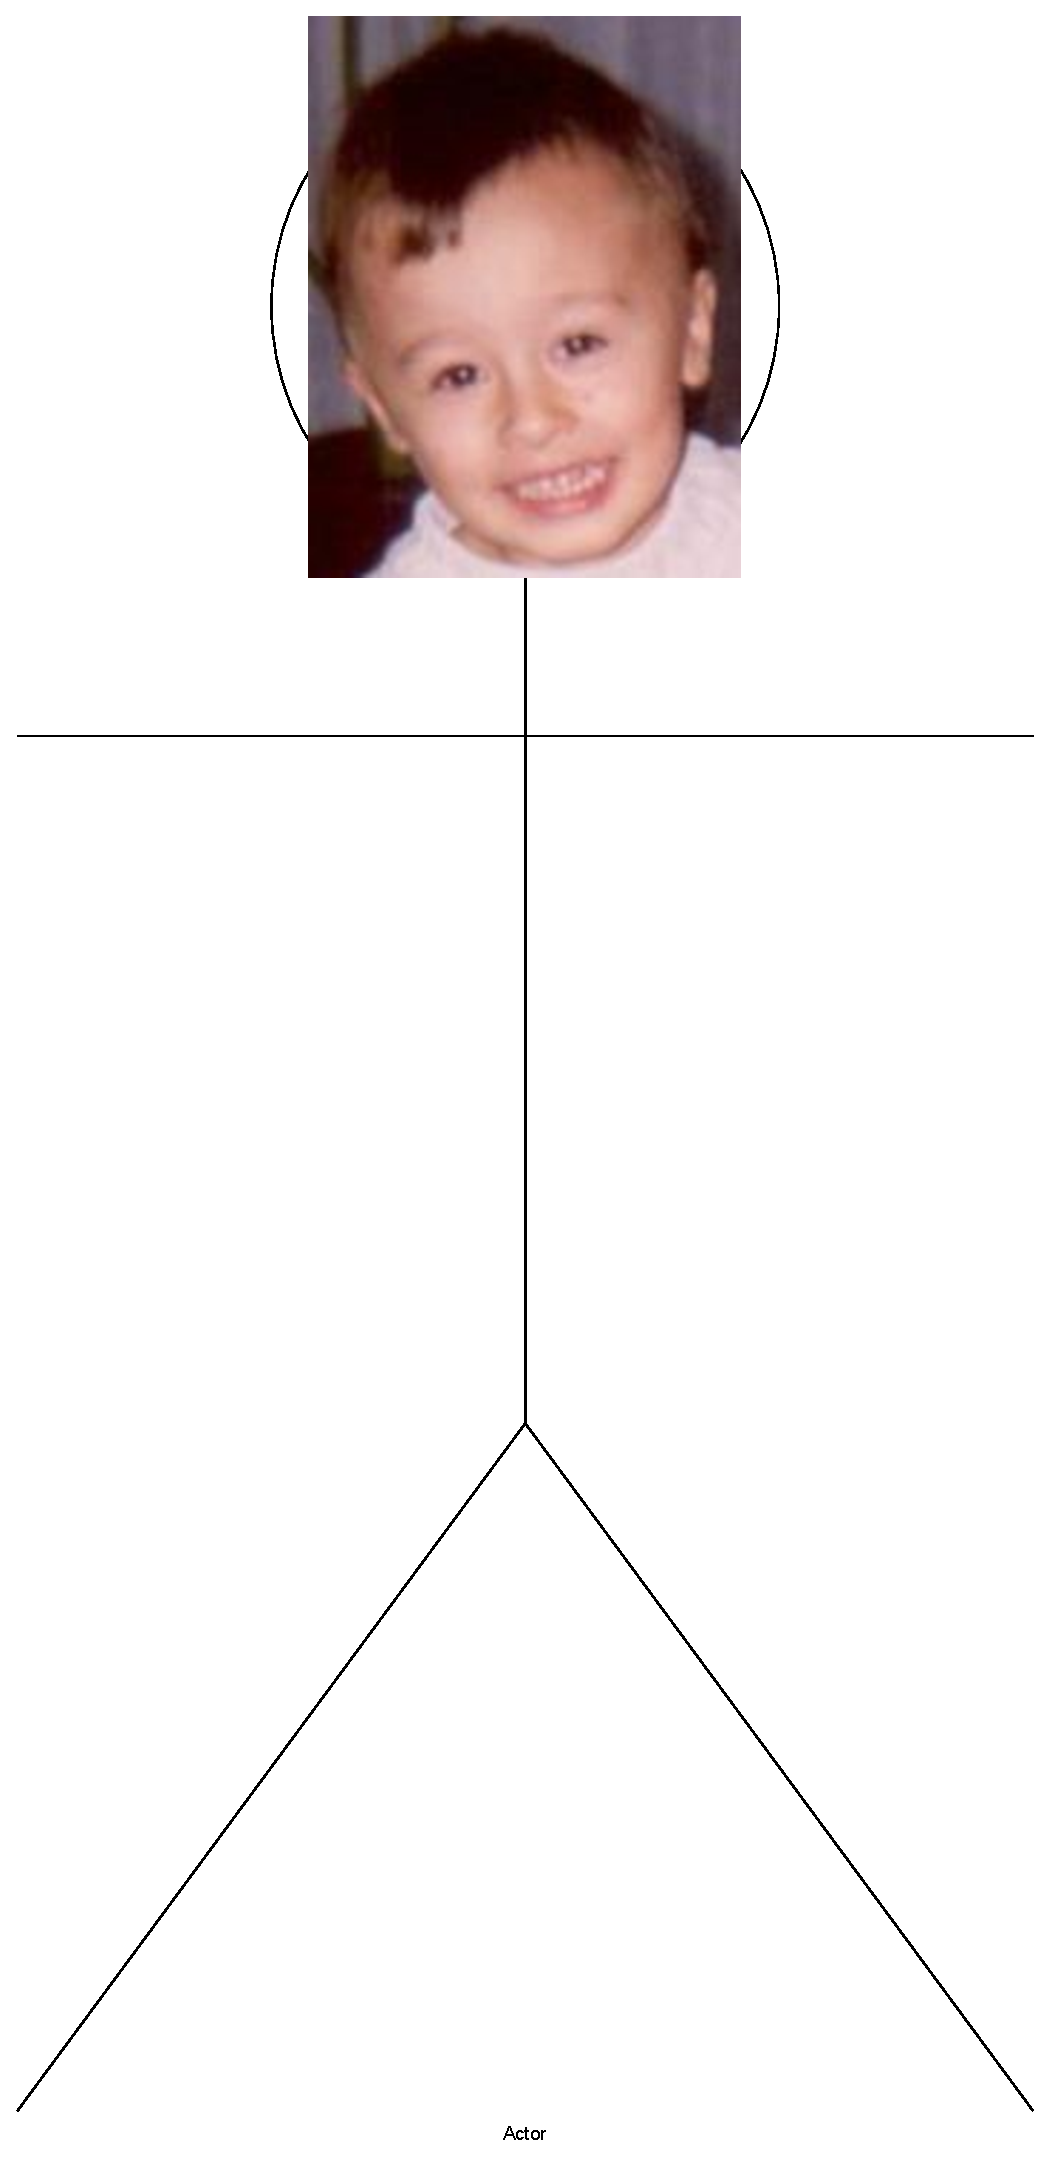
\includegraphics[width=0.4\textwidth]{fari}
%  \caption{Tatamata za distantnu zaštitu}
%  \label{fig:fari}
%\end{figure}

\section*{Smjernice za budući rad}

Sljedeće napomene i smjernice nisu razmatrane u ovom radu, a većina ih se može jednostavno implementirati i nadograditi na ovaj rad: 

\begin{enumerate}
    \item Kod ekstrakcije fazora mogu se pojaviti i frekvencije koje nisu umnožak fundamentalne frekvencije, a njih najčešće unose elektronički sklopovi. Njihove frekvencije se mogu identificirati i implementirati u metodi najmanjih kvadrata na jednostavan način.
    \item Kod proračuna zaštite nisu uzeti u obzir neki fenomeni. Zanemarene su paralelne grane $\pi$ ekvivalenta linije jer je i njihov utjecaj najčešće zanemariv, a može se umogućiti i njihov unos putem GUI-a. Također, mjerenja napona i struja nisu direktna već se vrše preko transformatora, pa se može omogućiti unos njihovih prenosnih odnosa preko GUI-a, te ih uzeti u obzir prilikom proračuna. Pored toga, nije implementirano mjerenje impedansi faza-faza jer se utjecaj posmatranih kvarova manifestirao na impedanse faza-zemlja.
    \item Moguće je analizirati i utjecaj drugih vrsta kvarova kao što je prekid faze, itd.
    \item Kod koji je implementiran vrši analizu na jednom periodu radi lakšeg i reprezentativnijeg prikaza rezultata, a moguće je proširiti analizu na širi ili kraći vremenski interval.
    \item U uvodnom poglavlju je naveden princip višestepene distantne zaštite, tj. zaštite više zona koji se može dodatno implementirati. Također, moguće je izvršiti kompenzaciju utjecaja drugih linija na liniju koja se štiti pomoću proračuna kratkih spojeva.  
\end{enumerate}